\titleformat{\chapter}[display]
{\centering\LARGE\bfseries} % Formatting style
{\chaptername\ \thechapter} % Chapter label
{20pt} % Spacing
{\LARGE} % Title formatting

\chapter{System Design}

This chapter describes the system design of the \emph{AI Content Factory}. It covers the architectural design, detailing the structural elements that manage the agentic graphs and client-server communications. It also details the data persistence layer and data access designs that enable state checkpoint recovery. Finally, it outlines the component layout, mapping the system's runtime workflows through UML activity diagrams, component diagrams, and data-flow diagrams, and discusses the design guidelines of the user interface.

\section{Architecture Design}

The architecture of the AI Content Factory is designed to support long-running, asynchronous, and stateful multi-agent workflows. Unlike traditional web applications that follow a request-response pattern, the proposed engine must coordinate background research tasks, semantic searches, interactive user reviews, parallel text generation, and video compilation. 

The system implements a client-server architecture. The server acts as a centralized engine, exposing API endpoints and managing the background agentic graph, while the client acts as an interactive dashboard.

\\begin{figure}[htbp]
	\centering
	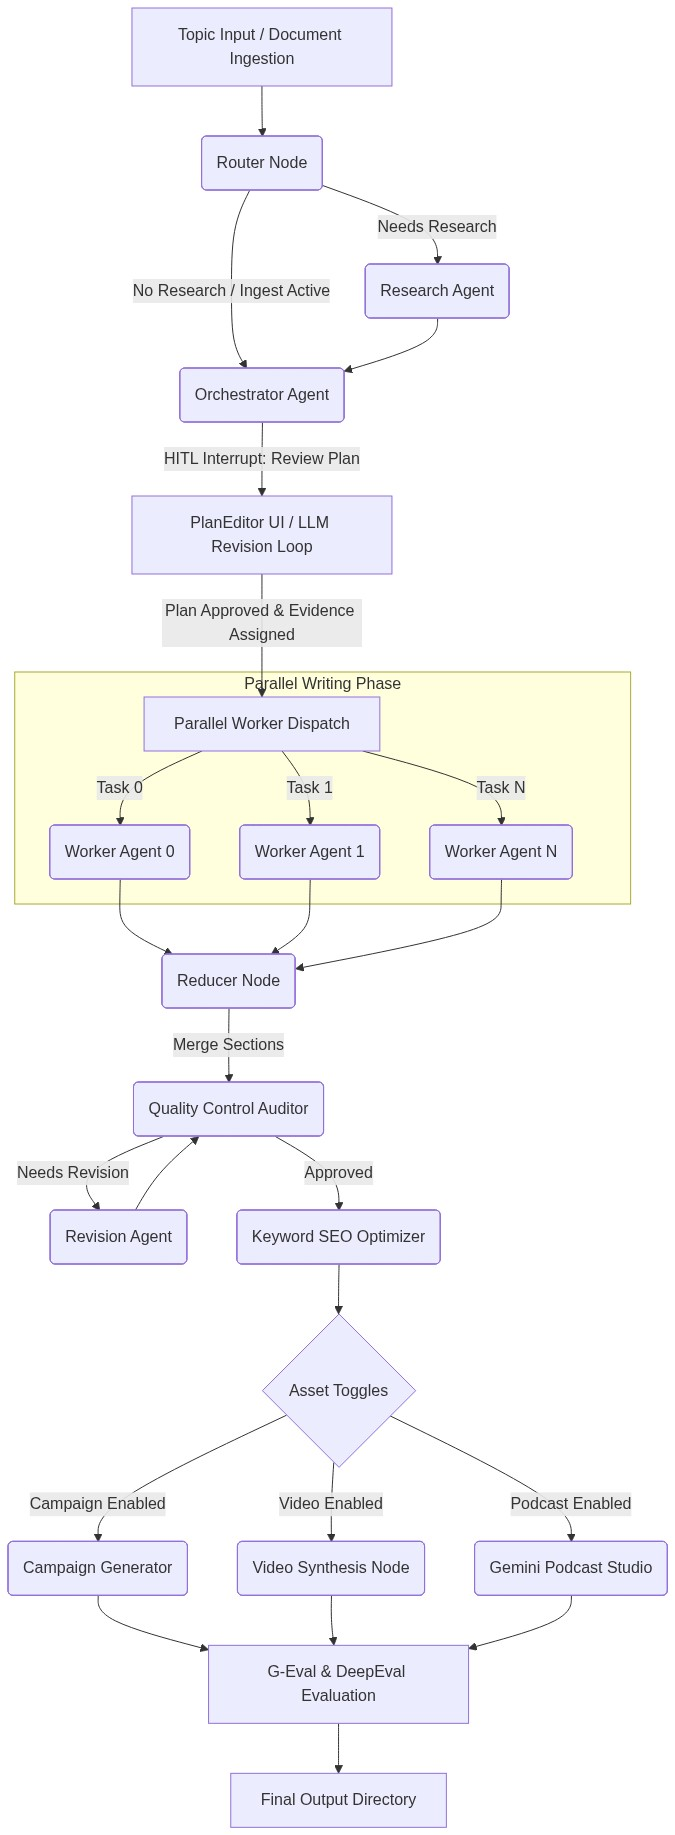
\includegraphics[width=1.0\textwidth, height = 0.75\textheight,keepaspectratio]{ArchitectureDiagram.png}
	\caption{General Architecture of Stateful Cognitive Agent Systems}
	\label{fig: General Architecture of Gaming System}
\end{figure}

Figure \ref{fig: General Architecture of Gaming System} shows the high-level architecture of stateful agent cognitive models. In this architecture, the LLM functions as the central reasoning core, surrounded by an environment state, active search tools, local files, and UI event loops.

The detailed runtime architecture of the proposed system is shown in Figure \ref{fig: Architecture Design Diagram}.

\begin{figure}[htbp]
	\centering
	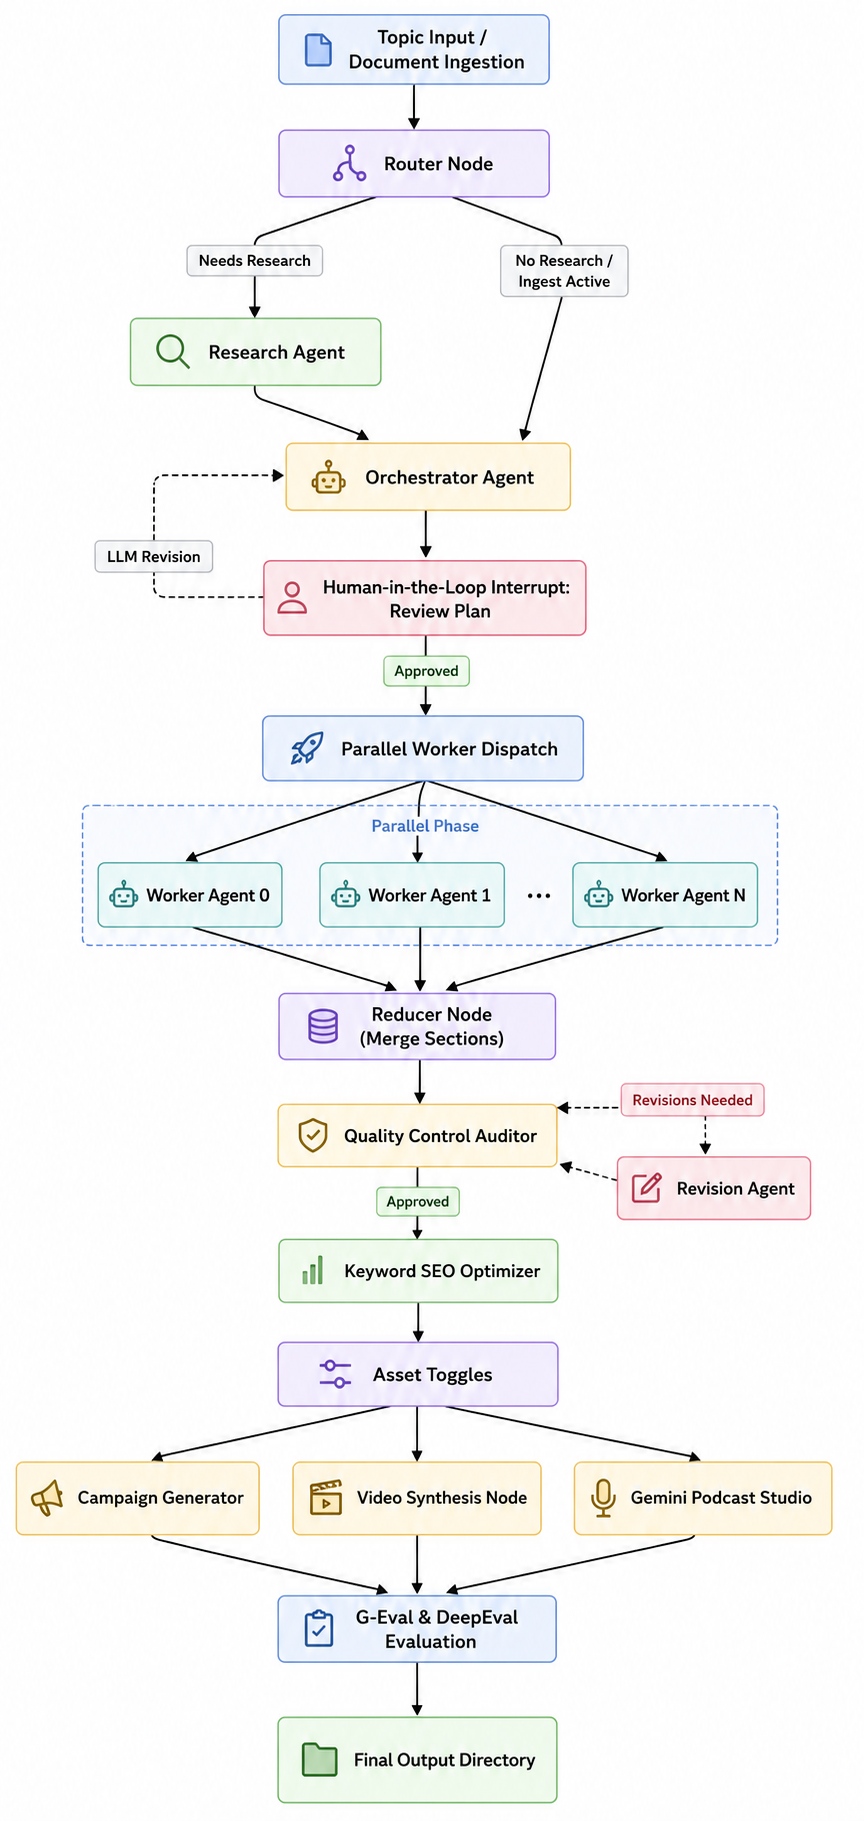
\includegraphics[width=1.0\textwidth, height = 0.75\textheight,keepaspectratio]{System Architecture Flow Diagram.png}
	\caption{Detailed Multi-Agent Interaction and Routing Graph}
	\label{fig: Architecture Design Diagram}
\end{figure}

The major architectural elements are defined as follows:
\begin{itemize}
	\item \textbf{LangGraph Engine:} The core workflow engine that executes the content generation graph. It routes states between agents and persists checkpoint transitions.
	\item \textbf{FastAPI Server:} The ASGI web application server that hosts REST API routes for job management and maintains real-time WebSocket connections to stream agent execution logs to the client.
	\item \textbf{Vite React Client:} The user interface dashboard that renders job lists, streams logs, provides the plan editor, and hosts media players.
	\item \textbf{Event Bus:} A central message broker that manages WebSocket subscriptions, routing agent thoughts and status updates to the UI in real-time.
\end{itemize}

\section{Data Persistence and Data Access Design}

A key requirement of the AI Content Factory is reliability. To ensure that intermediate progress is not lost during long runs, the system implements a structured database checkpointer and a relational storage schema.

\subsection{Data Persistence Design Details}
The system uses an SQLite database (`jobs.db`) to manage project data. The database schema consists of three major entities:
\begin{enumerate}
    \item \textbf{Job (State Run):} Stores the run ID, target topic, execution status (idle, running, paused, completed, failed), final article content, SEO density metrics, and execution metadata (token counts, total run cost, timestamps).
    \item \textbf{File (Grounding Documents):} Stores uploaded file data, containing name, file size, storage path, and status of semantic embedding generation.
    \item \textbf{Checkpoint (State Saver):} The binary storage table managed by LangGraph's checkpointer. It maps thread IDs to serialized state snapshots, including active variables and next nodes to run.
\end{enumerate}

Figure \ref{fig: Class Diagram} illustrates the class associations and relationships within the backend database model.

\begin{figure}[htbp]
	\centering
	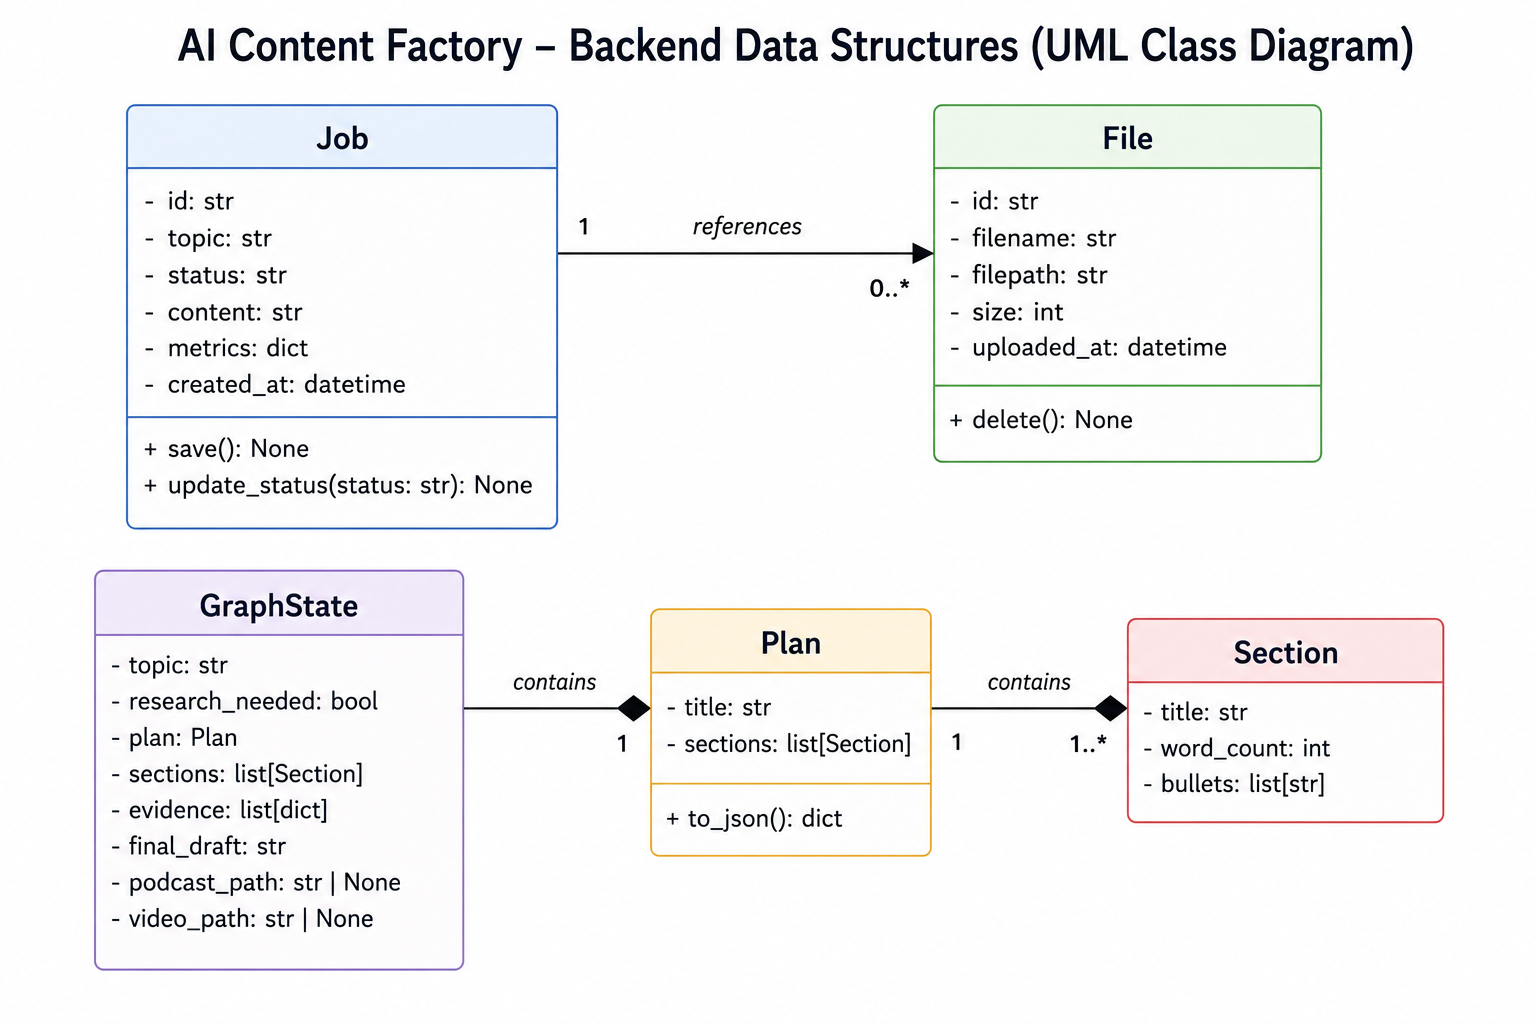
\includegraphics[width=1.0\textwidth, height = 0.75\textheight,keepaspectratio]{UML Class Diagram.png}
	\caption{Database Schema and Backend Model Class Association Diagram}
	\label{fig: Class Diagram}
\end{figure}

\subsection{Data Access Design Details}
Data access is managed through standardized data models and direct query interfaces to ensure clean code separation:
\begin{itemize}
	\item \textbf{Pydantic Schema Validation:} All incoming API requests (e.g., job creation, outline approvals) are validated against Pydantic models to ensure typing and validation gates are satisfied before database entry.
	\item \textbf{SQLite Connection Manager:} Handles database transaction loops, thread locks, and SQLite connections to prevent lock errors during concurrent read/write actions by parallel agent threads.
	\item \textbf{SqliteSaver Checkpointer:} An active checkpointer instance that intercepts every graph transition, serializes the current graph state using pickle/json, and writes the snapshot to the database.
\end{itemize}

\section{Component Design}

The system is structured as modular components, separating execution paths to keep code maintainable and extensible.

\begin{figure}[htbp]
	\centering
	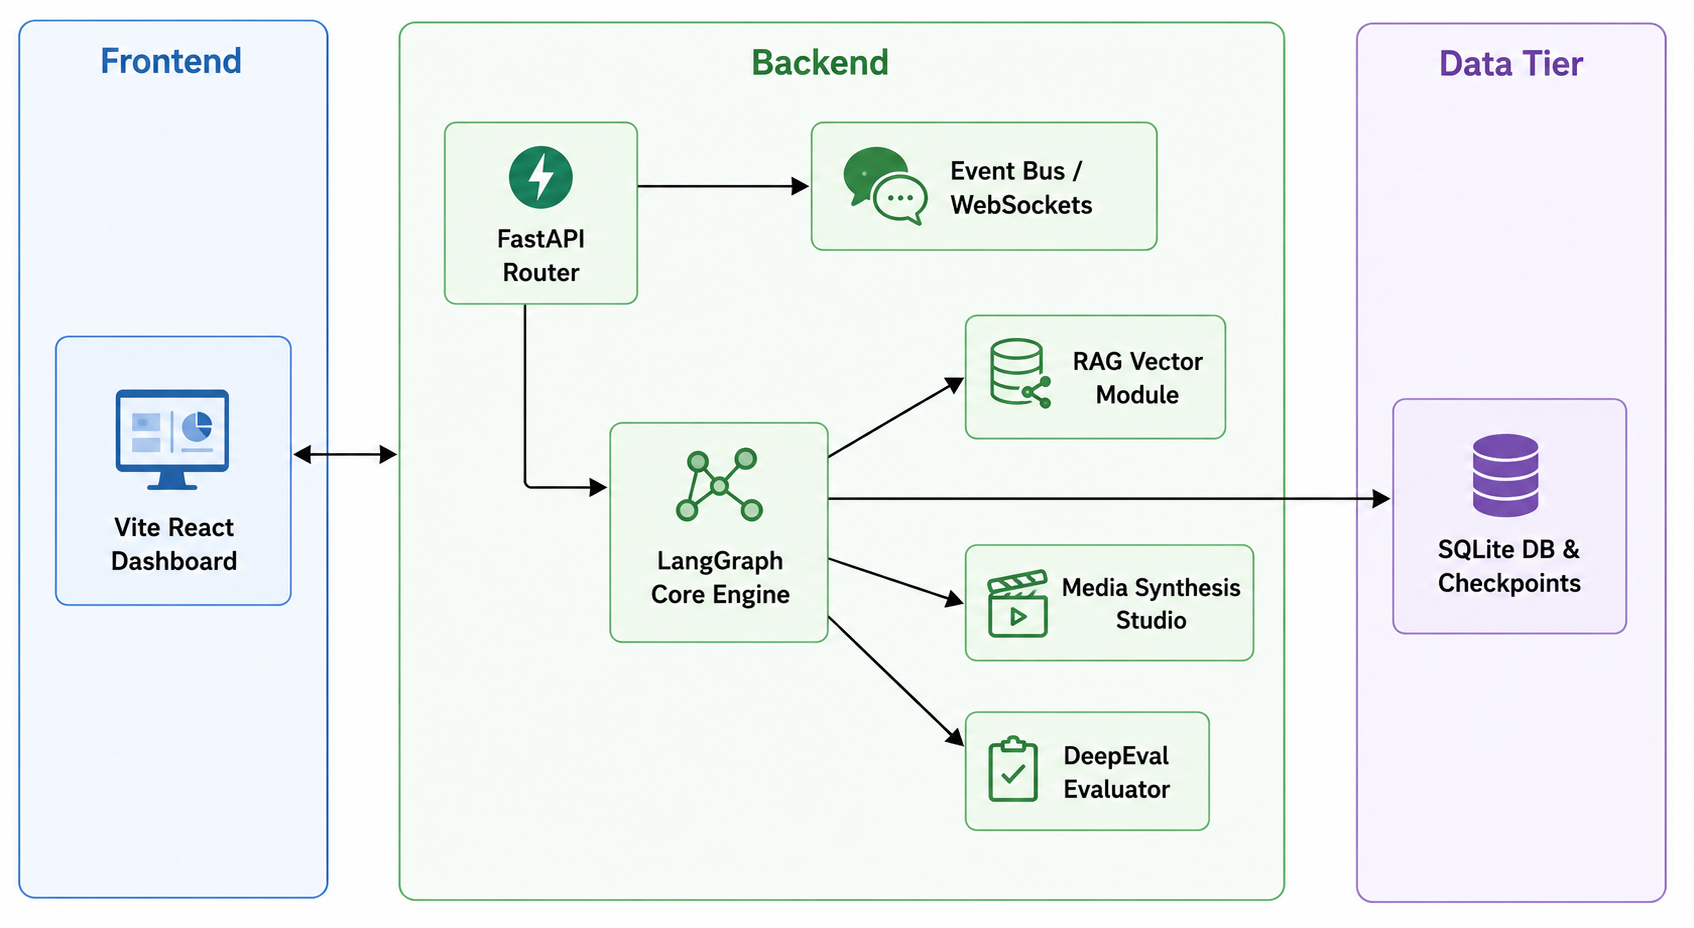
\includegraphics[width=1.0\textwidth, height = 0.75\textheight,keepaspectratio]{Component Diagram.png}
	\caption{Component Interaction Layout}
	\label{fig: Component Diagram}
\end{figure}

As shown in Figure \ref{fig: Component Diagram}, the backend is divided into specialized modules:
\begin{itemize}
    \item \textbf{Ingestion Module:} Handles text extraction and semantic chunking.
    \item \textbf{Graph Orchestration Module:} Coordinates agents, checks topics, and handles routing.
    \item \textbf{Media Synthesis Module:} Manages audio synthesis and video rendering.
    \item \textbf{Evaluation Module:} Handles scoring and writes DeepEval reports.
\end{itemize}

\subsection{System Workflow}
The workflow of the system is modeled as a cyclic state machine. The detailed execution logic is shown in Figure \ref{fig: Activity Diagram}.

\begin{figure}[htbp]
	\centering
    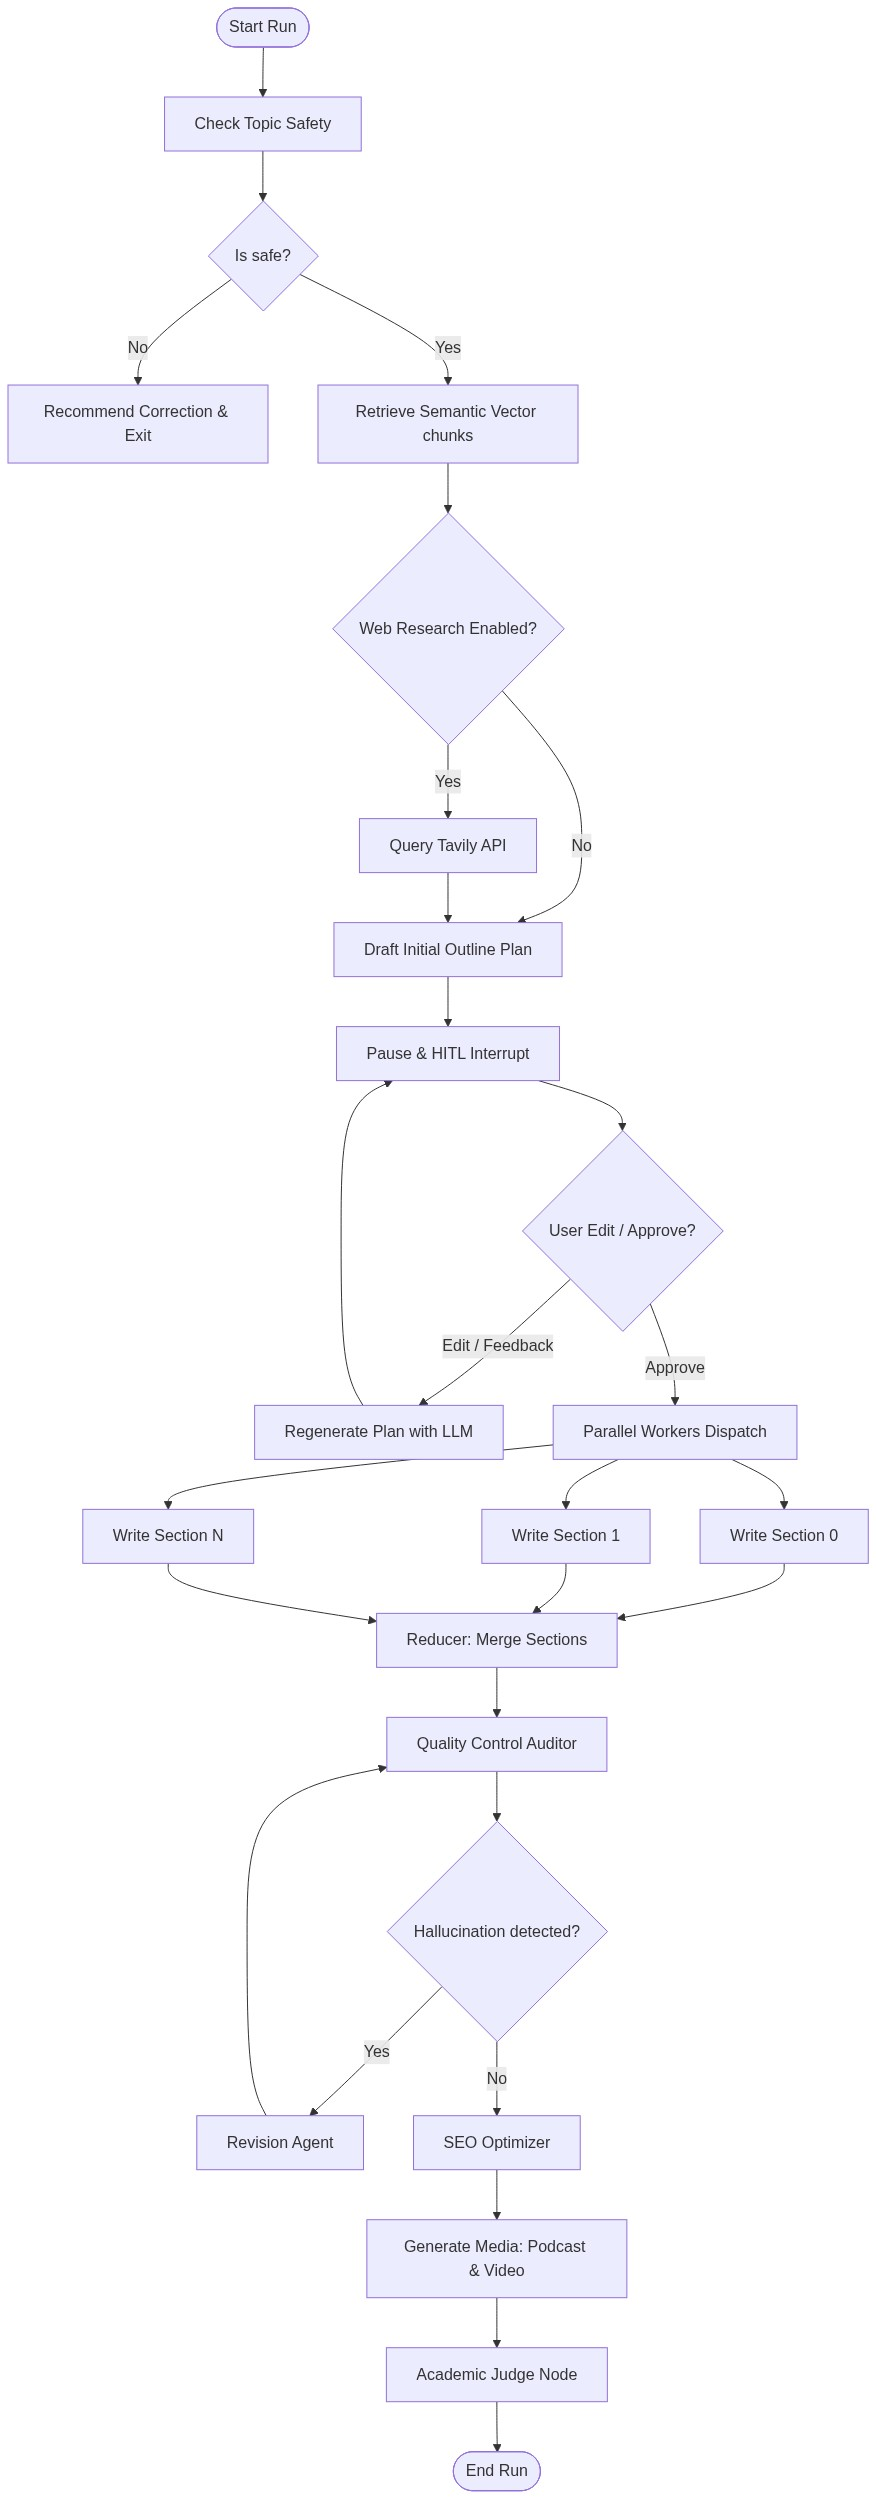
\includegraphics[width=1.0\textwidth, height = 0.8\textheight,keepaspectratio]{Activity Diagram.png}
	\caption{Workflow Transition and Logic Flow}
	\label{fig: Activity Diagram}
\end{figure}

The runtime execution follows these steps:
\begin{enumerate}
    \item The user inputs a topic and optional files via the React client.
    \item The backend validates safety constraints. If safe, it executes research queries and retrieves document embedding chunks.
    \item The Orchestrator drafts a plan and triggers a Human-in-the-Loop interrupt, saving state and pausing execution.
    \item The user edits or approves the plan on the client.
    \item The graph resumes, dispatching parallel workers to write the sections.
    \item The Reducer merges the text, and the Quality Control node audits it. If issues are found, the Revision node updates the draft.
    \item The SEO node optimizes keywords, then the media studio generates the podcast audio and composes the video.
    \item The Evaluation node runs G-Eval scoring, writes reports, and marks the status as completed.
\end{enumerate}

\subsection{Data Flow}
The exchange of data between the user, database, backend server, and third-party APIs is illustrated in the Level 0 Data Flow Diagram (Figure \ref{fig: Level 0 Data Flow Diagram}).

\begin{figure}[htbp]
	\centering
	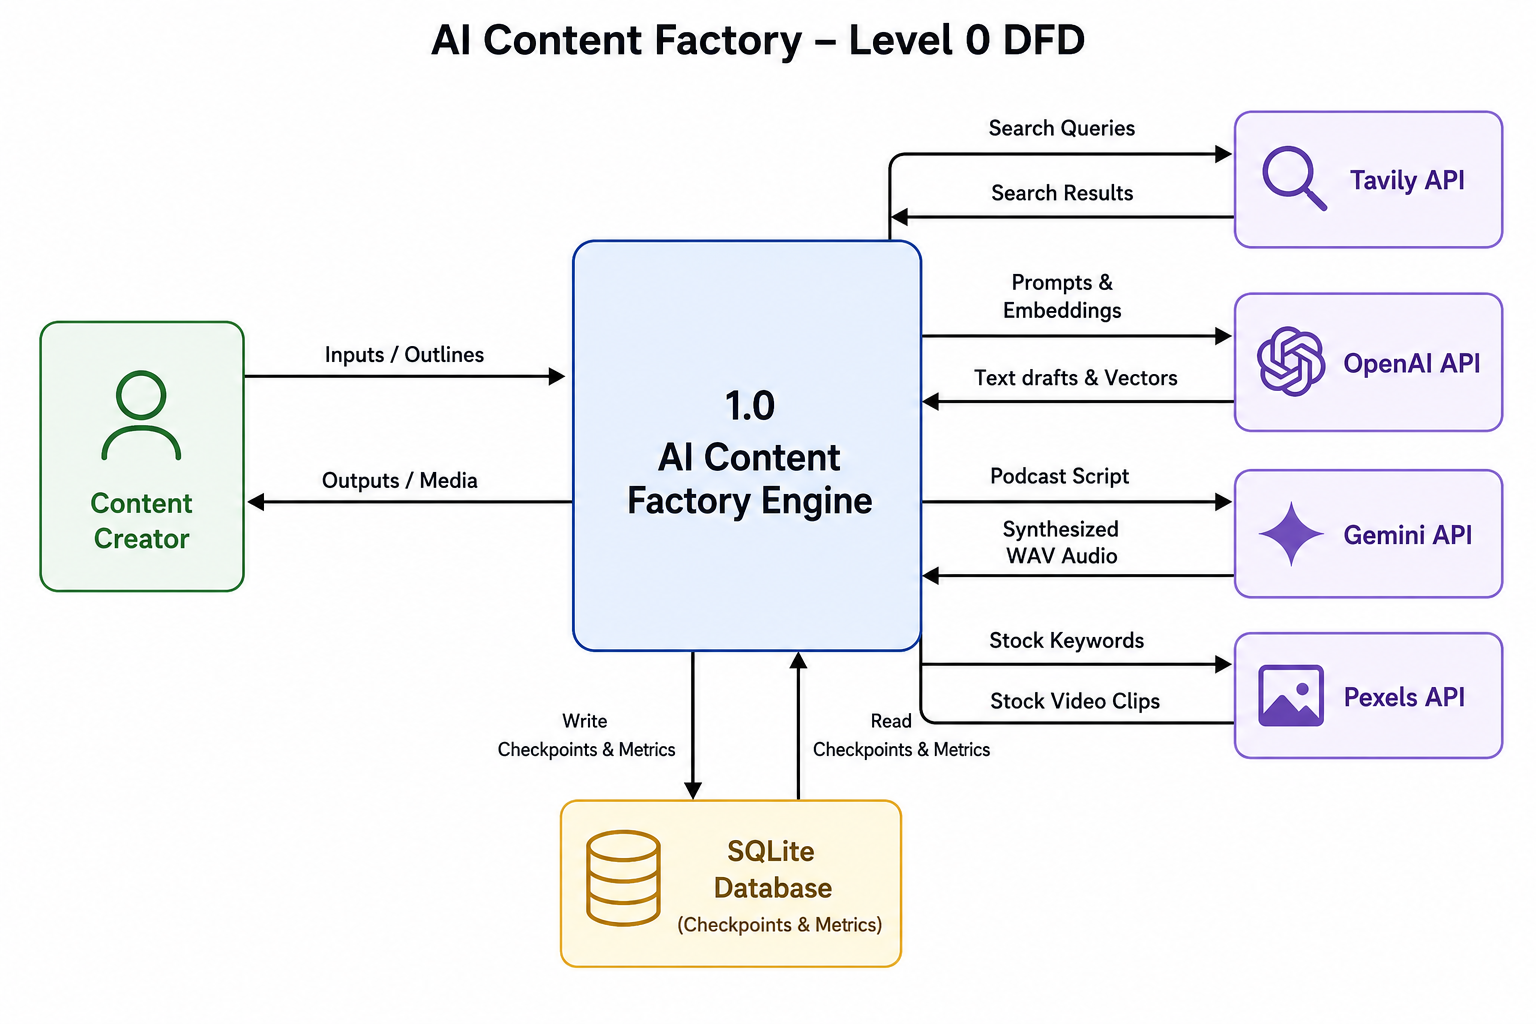
\includegraphics[width=1.0\textwidth, height = 0.75\textheight,keepaspectratio]{Data Flow Diagram (DFD Level 0).png}
	\caption{Level 0 DFD of the Content Engine}
	\label{fig: Level 0 Data Flow Diagram}
\end{figure}

As mapped in the DFD:
\begin{itemize}
    \item The user submits inputs and receives outputs (article, video, logs).
    \item The server queries external LLM and Search APIs, returning text responses, search data, and media files.
    \item The server reads and writes to the local SQLite database to persist logs and checkpoints.
\end{itemize}

\section{User-Interface Design}

The user interface of the AI Content Factory is designed to be interactive and transparent, providing users with visibility into backend agent actions.

\subsection{UI Layout Grid}
The UI uses a split-screen dashboard grid:
\begin{itemize}
    \item \textbf{Left Sidebar:} Shows a list of generated articles, navigation tabs, and system status indicators.
    \item \textbf{Center Console Tab:} Displays a terminal window showing real-time logs streamed via WebSockets, allowing the user to inspect agent thoughts.
    \item \textbf{Right Detail Tab:} Displays the generated markdown article, keyword density grids, HTML5 media players, and G-Eval scorecard overlays.
\end{itemize}

\subsection{Interactive Plan Editor Drawer}
During the Human-in-the-Loop phase, the UI opens a modal drawer showing:
\begin{itemize}
    \item A list of H2 headers. The user can drag and drop items to reorder them, edit titles, and adjust target word counts.
    \item Action buttons: \textbf{Approve} (sends updated state back to resume execution) and \textbf{Regenerate} (submits text feedback to the LLM to rewrite the plan).
\end{itemize}
This design ensures that the user has complete control over the content generation process.